\documentclass[11pt,a4paper]{article}
%%%----------------------------------------------------------------------------%%%
%%%----------------------------------------------------------------------------%%%
%%% 
%%% ### Packages 
%%%
%%%----------------------------------------------------------------------------%%%
%%%----------------------------------------------------------------------------%%%
\usepackage{amsmath, amsthm, amssymb, nccbbb, bm, dsfont, pifont, fontawesome, graphicx, varioref, enumitem, mathtools, listings, xcolor, cite}
\RequirePackage[round,authoryear]{natbib}
\RequirePackage[colorlinks,citecolor=blue,urlcolor=blue]{hyperref}
\usepackage[cal=boondox]{mathalfa}
%\usepackage[numbers]{natbib}
\setlength{\topmargin}{-1in}
\setlength{\textheight}{10.5in}
\setlength{\oddsidemargin}{-.6in}
\setlength{\textwidth}{7.5in}
\hypersetup{colorlinks=true, linkcolor=blue, citecolor=red, urlcolor=blue}

%%%----------------------------------------------------------------------------%%%
%%%----------------------------------------------------------------------------%%%
%%% 
%%% ### Code 
%%%
%%%----------------------------------------------------------------------------%%%
%%%----------------------------------------------------------------------------%%%
\usepackage{listings}
\lstset{escapeinside=| |}
\usepackage[usenames,dvipsnames]{color}  
\definecolor{mygray}{rgb}{0.99,0.99,0.99}
\definecolor{myblue}{rgb}{0.0, 0.23, 0.63}
\definecolor{myred}{rgb}{0.75, 0.0, 0.0}
\definecolor{mygreen}{rgb}{0.4, 0.69, 0.2}  
\lstnewenvironment{R}{\lstset{ 
  language=R,
  basicstyle=\footnotesize\ttfamily, 
  numbers=left,
  numberstyle=\tiny\color{black},
  stepnumber=1,
  numbersep=5pt,
  backgroundcolor=\color{mygray},
  showspaces=false, 
  showstringspaces=false,
  showtabs=false, 
  frame=single,  
  rulecolor=\color{black},
  tabsize=4,
  captionpos=b,
  breaklines=true,
  breakatwhitespace=false,
  keywordstyle=\ttfamily\bfseries\color{myblue},
  commentstyle=\ttfamily\bfseries\color{myred},
  stringstyle=\ttfamily\bfseries\color{mygreen}
} 
}{}

%New colors defined below
\definecolor{codegreen}{rgb}{0,0.6,0}
\definecolor{codegray}{rgb}{0.5,0.5,0.5}
\definecolor{codepurple}{rgb}{0.58,0,0.82}
\definecolor{backcolour}{rgb}{0.95,0.95,0.92}

%Code listing style named "mystyle"
\lstdefinestyle{mystyle}{
  backgroundcolor=\color{backcolour}, commentstyle=\color{codegreen},
  keywordstyle=\color{magenta},
  numberstyle=\tiny\color{codegray},
  stringstyle=\color{codepurple},
  basicstyle=\ttfamily\footnotesize,
  breakatwhitespace=false,         
  breaklines=true,                 
  captionpos=b,                    
  keepspaces=true,                 
  numbers=left,                    
  numbersep=5pt,                  
  showspaces=false,                
  showstringspaces=false,
  showtabs=false,                  
  tabsize=2
}

%"mystyle" code listing set
\lstset{style=mystyle}

%%%----------------------------------------------------------------------------%%%
%%%----------------------------------------------------------------------------%%%
%%% 
%%% ### Box
%%%
%%%----------------------------------------------------------------------------%%%
%%%----------------------------------------------------------------------------%%%
\usepackage{tcolorbox}
\tcbuselibrary{breakable}
\newtcolorbox{mybox}{colback=yellow!5!white, colframe=gray!60!black, breakable}
\newtcolorbox{mybox0}{colback=white, colframe=gray!60!black, breakable}
	

%%%----------------------------------------------------------------------------%%%
%%%----------------------------------------------------------------------------%%%
%%% 
%%% ### Theorem style structures 
%%%
%%%----------------------------------------------------------------------------%%%
%%%----------------------------------------------------------------------------%%%
\numberwithin{equation}{section}
\theoremstyle{plain}
\newtheorem{theorem}{Theorem}[section]
\newtheorem{lemma}[theorem]{Lemma}
\newtheorem{corollary}[theorem]{Corollary}
\newtheorem{proposition}[theorem]{Proposition}
\newtheorem{condition}{Condition}[section]
\newtheorem{definition}{Definition}[section]
\theoremstyle{definition}
\newtheorem{example}{Example}[section]
\newtheorem{exercise}{Exercise}[section]
\newtheorem{remark}{Remark}[section]
\newtheorem{remark0}{Remark}
\newtheorem{question}{Question}


%%%----------------------------------------------------------------------------%%%
%%%----------------------------------------------------------------------------%%%
%%% 
%%% ### Operators 
%%%
%%%----------------------------------------------------------------------------%%%
%%%----------------------------------------------------------------------------%%%
\newcommand{\pr}{\mathsf{P}} 
\newcommand{\E}{\mathsf{E}} 
\newcommand{\median}{\mathop{\mathsf{median}}}
\newcommand{\Cov}{{\mathsf{Cov}}} 
\newcommand{\Corr}{{\mathsf{Corr}}} 
\newcommand{\Var}{{\mathsf{Var}}}
\newcommand{\SD}{{\mathsf{SD}}}
\newcommand{\CV}{{\mathsf{CV}}}
\newcommand{\Bias}{{\mathsf{Bias}}}
\newcommand{\AMSE}{\operatorname{\mathsf{AMSE}}}
\newcommand{\MSE}{\operatorname{\mathsf{MSE}}}
\newcommand{\ARE}{\mathsf{ARE}}
\newcommand{\AV}{\mathsf{AV}}
\newcommand{\CRLB}{{\mathsf{CRLB}}}

\newcommand{\pCorr}{\text{P}}
\newcommand{\sCorr}{\text{S}}
\newcommand{\kCorr}{\text{K}}
\newcommand{\bdCorr}{\text{BD}}
\newcommand{\cCorr}{\text{C}}


\newcommand{\inD}{    \overset{ \textnormal{d}   }{\rightarrow} }
\newcommand{\inAS}{   \overset{ \textnormal{a.s.}   }{\rightarrow} }
\newcommand{\inP}{    \overset{ \textnormal{pr}    }{\rightarrow} }
\newcommand{\inLp}{   \overset{ \mathcal{L}^p }{\rightarrow} }
\newcommand{\inMSE}{  \overset{ \textnormal{qm} }{\rightarrow} }
\newcommand{\inQM}{   \overset{ \textnormal{qm} }{\rightarrow} }
\newcommand{\indep}{\protect\mathpalette{\protect\independenT}{\perp}}
\def\independenT#1#2{\mathrel{\rlap{$#1#2$}\mkern4mu{#1#2}}}
\newcommand{\iid}{\textsc{iid}} 
\newcommand{\simIID}{   \overset{ \iid   }{\sim} }
\newcommand{\simIND}{   \overset{ {\indep}   }{\sim} }


\newcommand{\Bern}{\textnormal{Bern}} 
\newcommand{\Unif}{\textnormal{Unif}} 
\newcommand{\Normal}{\textnormal{N}} 
\newcommand{\logNormal}{\textnormal{LN}} 
\newcommand{\Bin}{\textnormal{Bin}} 
\newcommand{\NB}{\textnormal{NB}} 
\newcommand{\HG}{\textnormal{HG}} 
\newcommand{\Geom}{\textnormal{Geom}} 
\newcommand{\Beta }{\textnormal{Beta}} 
\newcommand{\BetaBin}{\textnormal{Beta-Bin}}
\newcommand{\Ga}{\textnormal{Ga}} 
\newcommand{\Exp}{\textnormal{Exp}} 
\newcommand{\Expo}{\textnormal{Expo}} 
\newcommand{\Po}{\textnormal{Po}} 
\newcommand{\Multi}{\textnormal{Multi}} 
\newcommand{\student}{\textnormal{t}} 
\newcommand{\Cauchy}{\textnormal{Cauchy}} 
\newcommand{\Pareto}{\textnormal{Pareto}} 
\newcommand{\Laplace}{\textnormal{Laplace}} 
\newcommand{\Logistic}{\textnormal{Logistic}} 
\newcommand{\Dir}{\textnormal{Dir}} 
\newcommand{\DP}{\textnormal{DP}} 
\newcommand{\Inv}{\textnormal{Inv-}} 
\newcommand{\F}{\textnormal{F}} 
\newcommand{\sign}{\textnormal{sign}}
\newcommand{\rank}{\textnormal{rank}}


\newcommand{\RV}{\textsc{rv}}
\newcommand{\cdf}{\textsc{cdf}} 
\newcommand{\cgf}{\textsc{cgf}} 
\newcommand{\pdf}{\textsc{pdf}} 
\newcommand{\pmf}{\textsc{pmf}} 
\newcommand{\chf}{\textsc{chf}} 
\newcommand{\mgf}{\textsc{mgf}}
\newcommand{\EF}{\textsc{EF}}
\newcommand{\NEF}{\textsc{NEF}}
\newcommand{\MLE}{\textsc{mle}}
\newcommand{\MAP}{\textsc{MAP}}
\newcommand{\Med}{\textsc{Med}}
\newcommand{\MME}{\textsc{mme}}
\newcommand{\QME}{\textsc{qme}}
\newcommand{\UMVUE}{\textsc{umvue}}
\newcommand{\MPT}{\textsc{MPT}}
\newcommand{\UMPT}{\textsc{UMPT}}
\newcommand{\LRT}{\textsc{LRT}}


\newcommand{\diag}{\mathop{\mathrm{diag}}}
\newcommand{\tr}{\mathop{\mathrm{tr}}}
\newcommand{\T}{\mathop{\mathrm{T}}}
\DeclareMathOperator*{\argmin}{arg\,min}
\DeclareMathOperator*{\argmax}{arg\,max}
\DeclareMathOperator{\sgn}{sgn}
\DeclareMathOperator{\logit}{logit}
\DeclareMathOperator{\expit}{expit}
\newcommand{\dd}{\textnormal{d}}


\newcommand{\lva}{{\color{myred}\ding{73}\ding{73}\ding{73}}}
\newcommand{\lvb}{{\color{myred}\ding{72}\ding{73}\ding{73}}}
\newcommand{\lvc}{{\color{myred}\ding{72}\ding{72}\ding{73}}}
\newcommand{\lvd}{{\color{myred}\ding{72}\ding{72}\ding{72}}}
\newcommand{\optional}{\noindent{\color{myblue}\faScissors}}
\newcommand{\Solution}{\noindent{\color{myblue}{{\textsc{Solution}}:~$\Big.$}}}
\newcommand{\take}{\noindent{\color{myblue}\faPaperPlaneO~\underline{\bf Takeaway}:~$\Big.$}}

% widecheck 
\DeclareFontFamily{U}{mathx}{\hyphenchar\font45}
\DeclareFontShape{U}{mathx}{m}{n}{
      <5> <6> <7> <8> <9> <10>
      <10.95> <12> <14.4> <17.28> <20.74> <24.88>
      mathx10
      }{}
\DeclareSymbolFont{mathx}{U}{mathx}{m}{n}
\DeclareFontSubstitution{U}{mathx}{m}{n}
\DeclareMathAccent{\widecheck}{0}{mathx}{"71}
\DeclareMathAccent{\wideparen}{0}{mathx}{"75}

\def\cs#1{\texttt{\char`\\#1}}

\newcounter{magicrownumbers}
\newcommand\rownumber{\stepcounter{magicrownumbers}\arabic{magicrownumbers}}


%------------------------------------------------------------------------------



\begin{document}
    % Page 0 for names and table of contents
    \thispagestyle{empty}
    \pagenumbering{gobble} 
    \title{\textsc{RMSC 4002} -- Financial Data Analytics with Machine Learning \\ Group Project}
    \author{
        CHOI Sen Hei (SID: \texttt{1155109412}) \\
        IEONG Hei (SID: \texttt{1155104271}) \\
        LAM Wai Chui (SID: \texttt{1155152095}) \\
        LAU Chiu Tan (SID: \texttt{1155108960}) \\
        LAW Yiu Leung Eric (SID: \texttt{1155149315})
    }
    \date{\today}
    \maketitle
    
    \tableofcontents
    \newpage
    
    
    % Section 1
    \pagenumbering{arabic}
    \setcounter{page}{1}
    
    \section{Principal Component Analysis Factor Models and Recommender Systems}
    \subsection{Pricipal Component Analysis (PCA)}
    
    
    % Section 2
    \newpage
    \section{Classification / Decision and Regression Trees}
    In this section, we are going to use Decision Trees and Random Forest methods to predict binary response variable.
    
    \subsection{Dataset}
    For the dataset, we use \href{https://archive.ics.uci.edu/ml/datasets/bank+marketing}{Bank Marketing Data Set} from  \href{https://archive.ics.uci.edu/ml/index.php}{UCI Machine Learning Repository}.
    The data is related with direct marketing campaigns of a Portuguese banking institution. The marketing campaigns were based on phone calls. Often, more than one contact to the same client was required, in order to access if the product (bank term deposit) would be ('yes') or not ('no') subscribed \cite{MORO201422}. There are total 21 variables (including y, the response variable), 41188 valid records.
    
    \subsection{Feature Description}
    There are 20 explanatory variables, including numerical and categorical variables:
    
    \begin{table}[h]
        \begin{minipage}{.5\linewidth}
            \centering
            \begin{tabular}{r c c}
                 & Feature & Type \\
                \hline \hline
                \rownumber & age & numeric \\
                \rownumber & job & categorical \\
                \rownumber & marital & categorical \\
                \rownumber & education & categorical \\
                \rownumber & default & categorical \\
                \rownumber & housing & categorical \\
                \rownumber & loan & categorical \\
            \end{tabular}
            \caption{Bank client data}\label{tab:bank.client}
        \end{minipage}%
        \begin{minipage}{.5\linewidth}
            \centering
            \begin{tabular}{r c c}
                 & Feature & Type \\
                \hline \hline
                \rownumber & contact & categorical \\
                \rownumber & month & categorical \\
                \rownumber & day\_of\_week & categorical \\
                \rownumber & duration & numerical \\
            \end{tabular}
            \caption{Related with the last contact of the current campaign}\label{tab:last.contact}
        \end{minipage}
    \end{table}
    
    \begin{table}[h]
        \begin{minipage}{.5\linewidth}
            \centering
            \begin{tabular}{r c c}
                 & Feature & Type \\
                \hline \hline
                \rownumber & campaign & numeric \\
                \rownumber & pdays & numerical \\
                \rownumber & previous & numerical \\
                \rownumber & poutcome & categorical \\
            \end{tabular}
            \caption{Other attributes}\label{tab:other}
        \end{minipage}%
        \begin{minipage}{.5\linewidth}
            \centering
            \begin{tabular}{r c c}
                 & Feature & Type \\
                \hline \hline
                \rownumber & emp.var.rate & numerical \\
                \rownumber & cons.price.idx & numerical \\
                \rownumber & cons.conf.idx & numerical \\
                \rownumber & euribor3m & numerical \\
                \rownumber & nr.employed & numerical \\
            \end{tabular}
            \caption{social and economic context attributes}\label{tab:soc.econ}
        \end{minipage}
    \end{table}
    
    \subsection{Project Description}
    We are going to perform an analysis in \textbf{topic 6: Classification / Decision and Regression Trees}. We will use \nameref{decision_trees} and \nameref{random_forest} to do classification on response variable \textbf{y}, i.e. whether the client subscribed a term deposit. \\
    \\
    The following steps will be performed to complete this section:
    \begin{enumerate}
        \item process data explanatory data analysis (EDA)
        \item data preparation for modeling
        \item visualization of random forest and decision tree
        \item cross validation and grid search
        \item comparison of the performance of random forest and decision tree
        \item conclusions
    \end{enumerate}
    
    \subsection{Process Data and Explanatory Data Analysis (EDA)}
    Import libraries
\begin{lstlisting}[language = Python]
import pandas as pd
import numpy as np
from datetime import datetime
import time
import gc
from IPython.display import display
import warnings
warnings.filterwarnings("ignore")

from sklearn.model_selection import train_test_split, GridSearchCV, StratifiedKFold
from sklearn.ensemble import RandomForestClassifier
from sklearn import tree
from sklearn.pipeline import Pipeline
from sklearn.metrics import roc_curve, roc_auc_score
import category_encoders as ce

import plotly.graph_objs as go
import matplotlib.pyplot as plt
\end{lstlisting}
\quad \\
    Loading data and a short explanatory data analysis
\begin{lstlisting}[language = Python]
# Process data
data = pd.read_csv('../../data/bank-additional-full.csv', sep=';')
display(data.sample(10))
display('There are {} observations with {} features'.format(data.shape[0], data.shape[1]))
\end{lstlisting}
\quad \\
    \begin{tabular}{lrlllllllcl}
        {} &  age &          job &   marital &          education & default & housing & loan &   contact & ... & y\\
        
        35666 &   58 &   management &   married &  university.degree &      no &      no &   no &  cellular & ... & no \\
        36531 &   48 &       admin. &   married &  university.degree &      no &     yes &   no &  cellular & ... & yes \\
        38676 &   73 &      retired &   married &  university.degree &      no &      no &  yes &  cellular & ... & yes \\
        15146 &   49 &   technician &  divorced &        high.school &      no &      no &   no &  cellular & ... & no \\
        33230 &   33 &  blue-collar &    single &           basic.6y &      no &     yes &   no &  cellular & ... & no \\
    \end{tabular} \\ \\
    \texttt{There are 41188 observations with 21 features}
    
    \subsubsection{Categorical Variables}
\begin{lstlisting}[language = Python]
# Function of plotting the categorical values disribution
def plot_bar(column):
    temp = pd.DataFrame()  #create a tremp dataframe
    temp['Not_deposit'] = data[data['y'] == 'no'][column].value_counts() # count the value when y = no
    temp['Deposit'] = data[data['y'] == 'yes'][column].value_counts() # count the value when y = yes

    temp = temp.apply(lambda x: x / x.sum(), axis = 1) * 100
    temp.sort_values("Deposit", inplace = True)
    temp.plot(
        kind = "barh", 
        stacked = True, 
        title = "Percentage Stacked Bar Graph for {}".format(column), 
        mark_right = True
    ).legend(loc = "center left", bbox_to_anchor = (1, 0.5))

    plt.savefig("../../plot/classification/{}.pdf".format(column), bbox_inches = "tight")
    plt.show();

plot_bar('job'), plot_bar('marital'), plot_bar('education'), plot_bar('contact'), plot_bar('loan'), plot_bar('housing')
\end{lstlisting}
    
    \begin{figure}%
        \centering
        \subfloat[job]{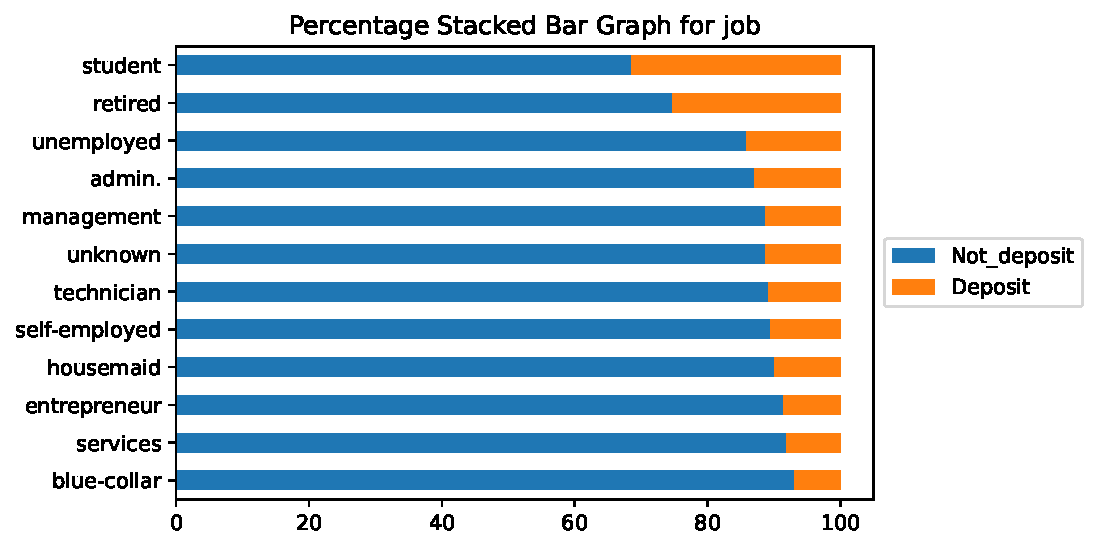
\includegraphics[scale=0.4]{plot/classification/job.pdf}}%
        \qquad
        \subfloat[marital]{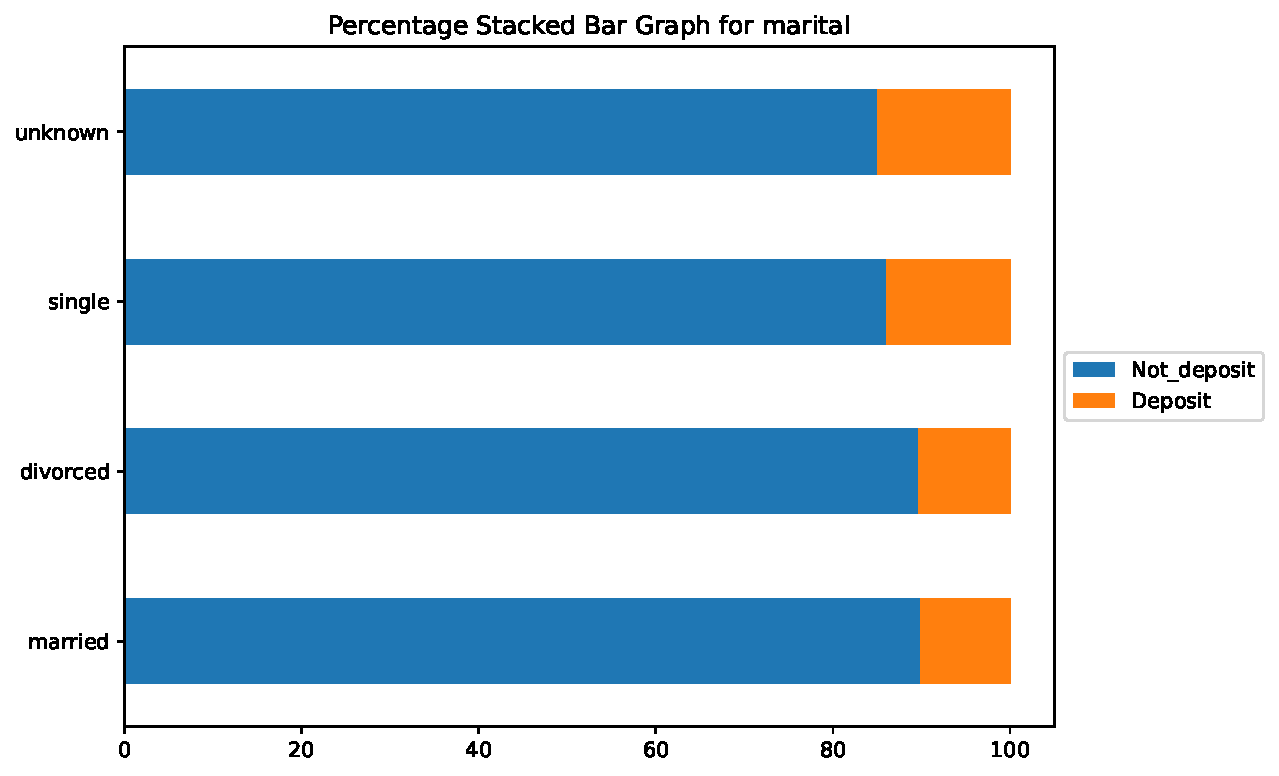
\includegraphics[scale=0.4]{plot/classification/marital.pdf}}%
    
        \subfloat[education]{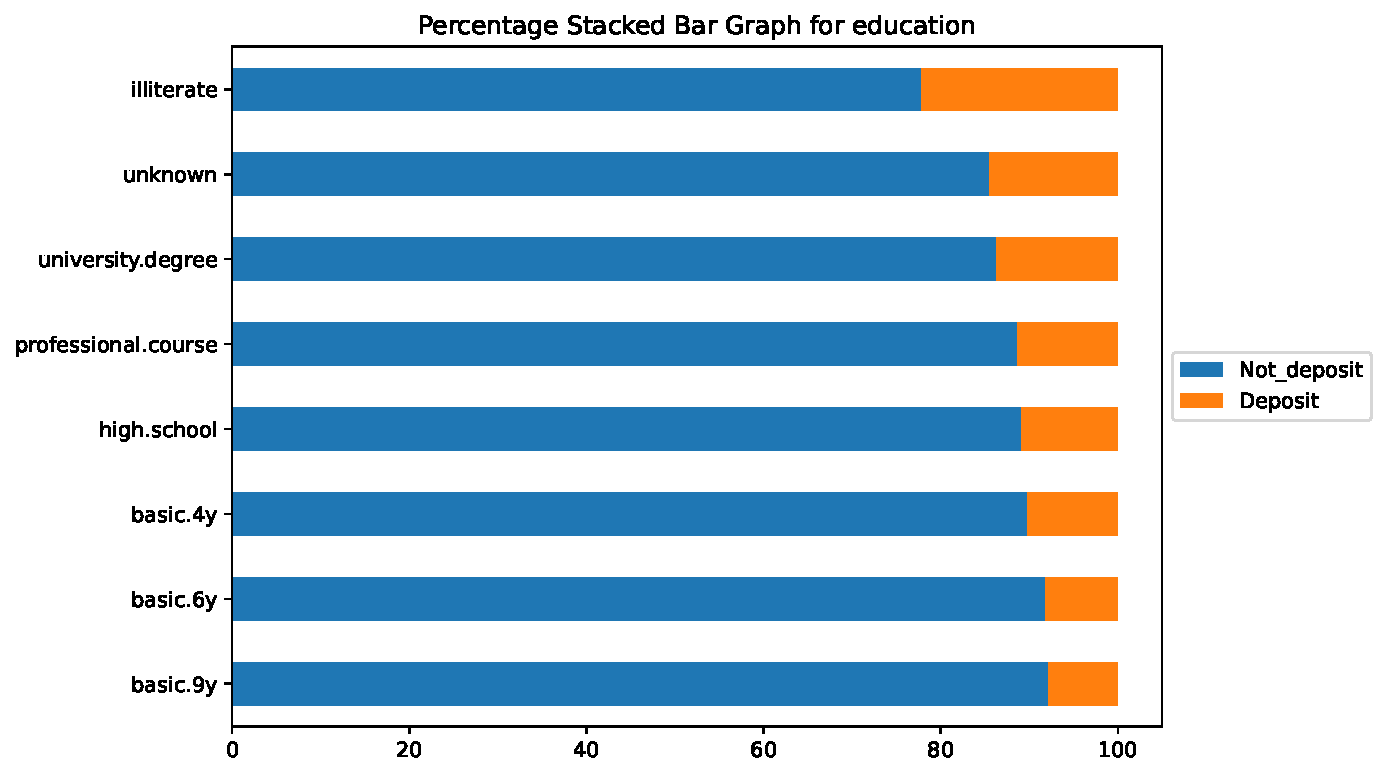
\includegraphics[scale=0.4]{plot/classification/education.pdf}}%
        \qquad
        \subfloat[contact]{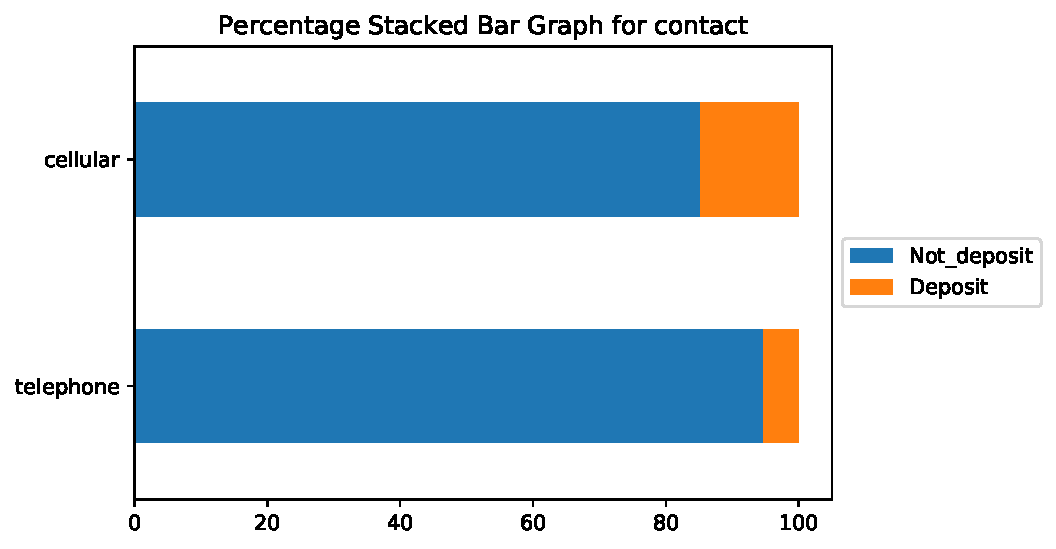
\includegraphics[scale=0.4]{plot/classification/contact.pdf}}%
        
        \subfloat[loan]{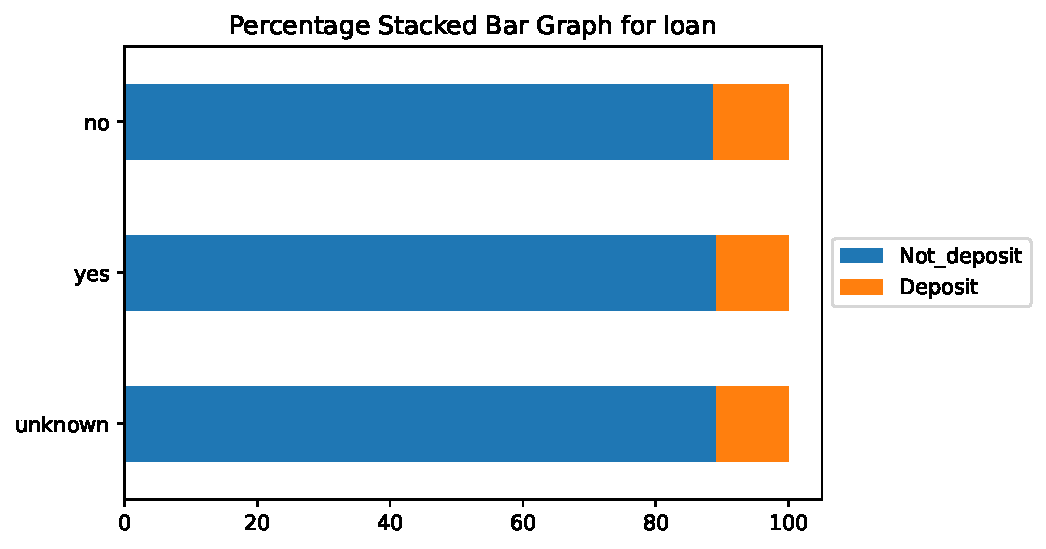
\includegraphics[scale=0.4]{plot/classification/loan.pdf}}%
        \qquad
        \subfloat[contact]{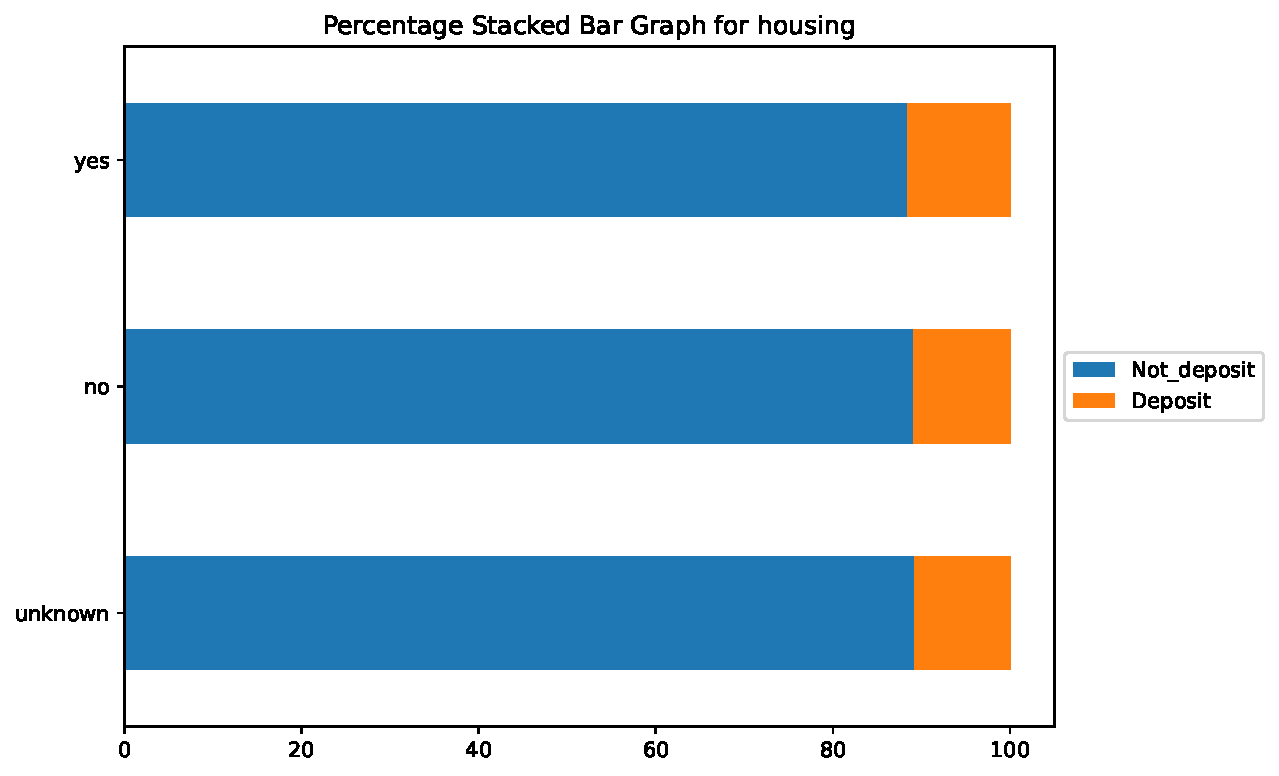
\includegraphics[scale=0.4]{plot/classification/housing.pdf}}%
    \end{figure}
    \quad \\
    \textbf{Summary of Categorical Variables:}
    \begin{enumerate}
        \item When job types are retired and student, the proportions of opening the deposit are high as well.
        \item 
    \end{enumerate}
    
    \subsubsection{Numerical Variables}
\begin{lstlisting}[language = Python]
corr = data.corr()
corr.style.background_gradient(cmap = 'Spectral')
\end{lstlisting}
    \quad \\
    {\tiny
        \begin{tabular}{lrrrrrrrrrrr}
            {} &     age &  duration &  campaign &   pdays &  previous &  emp.var.rate &  cons.price.idx &  cons.conf.idx &  euribor3m &  nr.employed &       y \\
            
            age            &  1.0000 &   -0.0009 &    0.0046 & -0.0344 &    0.0244 &       -0.0004 &          0.0009 &         0.1294 &     0.0108 &      -0.0177 &  0.0304 \\
            duration       & -0.0009 &    1.0000 &   -0.0717 & -0.0476 &    0.0206 &       -0.0280 &          0.0053 &        -0.0082 &    -0.0329 &      -0.0447 &  0.4053 \\
            campaign       &  0.0046 &   -0.0717 &    1.0000 &  0.0526 &   -0.0791 &        0.1508 &          0.1278 &        -0.0137 &     0.1351 &       0.1441 & -0.0664 \\
            pdays          & -0.0344 &   -0.0476 &    0.0526 &  1.0000 &   -0.5875 &        0.2710 &          0.0789 &        -0.0913 &     0.2969 &       0.3726 & -0.3249 \\
            previous       &  0.0244 &    0.0206 &   -0.0791 & -0.5875 &    1.0000 &       -0.4205 &         -0.2031 &        -0.0509 &    -0.4545 &      -0.5013 &  0.2302 \\
            emp.var.rate   & -0.0004 &   -0.0280 &    0.1508 &  0.2710 &   -0.4205 &        1.0000 &          0.7753 &         0.1960 &     0.9722 &       0.9070 & -0.2983 \\
            cons.price.idx &  0.0009 &    0.0053 &    0.1278 &  0.0789 &   -0.2031 &        0.7753 &          1.0000 &         0.0590 &     0.6882 &       0.5220 & -0.1362 \\
            cons.conf.idx  &  0.1294 &   -0.0082 &   -0.0137 & -0.0913 &   -0.0509 &        0.1960 &          0.0590 &         1.0000 &     0.2777 &       0.1005 &  0.0549 \\
            euribor3m      &  0.0108 &   -0.0329 &    0.1351 &  0.2969 &   -0.4545 &        0.9722 &          0.6882 &         0.2777 &     1.0000 &       0.9452 & -0.3078 \\
            nr.employed    & -0.0177 &   -0.0447 &    0.1441 &  0.3726 &   -0.5013 &        0.9070 &          0.5220 &         0.1005 &     0.9452 &       1.0000 & -0.3547 \\
            y              &  0.0304 &    0.4053 &   -0.0664 & -0.3249 &    0.2302 &       -0.2983 &         -0.1362 &         0.0549 &    -0.3078 &      -0.3547 &  1.0000 \\
        \end{tabular}
    } \\ \\
    \textbf{Summary of Numerical Variables:}
    \begin{itemize}
        \item \texttt{duration} is the highest correlated variable with target feature (0.4053).
        \item \texttt{nr.employed, pdays, euribor3m} are also highly correlated with target feature.
    \end{itemize}
    
    
    \subsection{Data Preparation for modeling}
    \subsubsection{Transformation for Categorical Variables}
    Since this dataset contains a lot of categorical variables and the number of weakly correlated numeric variables is small, therefore, we use one-hot encoding to transform categorical data.  While for binary categorical variables, we transform it into binary number accordingly (0 and 1). \\
    For \texttt{job, marital, education, month, day\_of\_week}, we use one-hot encoding to transform these variables since they have more than 3 types of possible options. \\
    Moreover, some variables contain missing data, labeled as \texttt{unknown} or \texttt{nonexistent}, we treat it as 0 (i.e. no) in general.
    
\begin{lstlisting}[language = Python]
# Fucntion of One Hot Encoding
def encode(data, col):
    return pd.concat([data, pd.get_dummies(col, prefix=col.name)], axis=1)

# Replacing values with binary number
data.contact = data.contact.map({'cellular': 0, 'telephone': 1}).astype('uint8') 
data.loan = data.loan.map({'unknown': 0, 'no' : 0, 'yes': 1}).astype('uint8')
data.default = data.default.map({'unknown': 0,'no': 0, 'yes': 1}).astype('uint8')
data.housing = data.housing.map({'unknown': 0, 'no' : 0,'yes': 1}).astype('uint8')
# binary if were was an outcome of marketing campane
data.poutcome = data.poutcome.map({'nonexistent':0, 'failure':0, 'success':1}).astype('uint8') 

# One Hot encoding of 3 variable 
data = encode(data, data.job)
data = encode(data, data.month)
data = encode(data, data.day_of_week)

# Drop tranfromed features
data.drop(['job','month', 'day_of_week'], axis=1, inplace=True)

'''Drop the dublicates'''
data.drop_duplicates(inplace=True) 

# Save target variable as y
y = data.y
# Create target encoder object and transoform marital and education
target_encode = ce.target_encoder.TargetEncoder(cols=['marital', 'education']).fit(data, y)
dataset_prepared = target_encode.transform(data)
# Drop target variable
dataset_prepared.drop('y', axis=1, inplace=True)

display(dataset_prepared.sample(10))
display('There are {} observations with {} features in the prepared dataset'.format(dataset_prepared.shape[0], dataset_prepared.shape[1]))
\end{lstlisting}
    \quad \\
    \begin{tabular}{lrrrrrrrrr}
        {} &  age &   marital &  education &  default &  housing &  loan &  contact &  duration &  campaign \\
        
        29851 &   52 &  0.103231 &   0.137219 &        0 &        1 &     0 &        1 &        70 &         4 \\
        15768 &   39 &  0.140090 &   0.113550 &        0 &        0 &     0 &        0 &        65 &         2 \\
        38033 &   76 &  0.101569 &   0.102515 &        0 &        1 &     0 &        0 &       259 &         2 \\
        27290 &   37 &  0.140090 &   0.137219 &        0 &        1 &     1 &        0 &       661 &         1 \\
        30685 &   34 &  0.101569 &   0.078246 &        0 &        1 &     0 &        0 &       332 &         1 \\
    \end{tabular} \\ \\
    \texttt{There are 41174 observations with 44 features in the prepared dataset}
    
    
    \subsubsection{Splitting Training Dataset and Testing Dataset}
\begin{lstlisting}[language = Python]
# Set global random seed
random_state = 4002
# split data
x_train, x_test, y_train, y_test = train_test_split(dataset_prepared, y, test_size=0.2, random_state=random_state)
\end{lstlisting}
    
    
    \subsection{Decision Trees} \label{decision_trees}
    Setting the depth of decision tree to 3, to plot a simplified decision tree.
\begin{lstlisting}[language = Python]
# Set max_depth = 3 to keep the size of the tree small for ploting graph
dt = tree.DecisionTreeClassifier(max_depth=3, random_state=random_state)
dt.fit(x_train, y_train)
plt.figure(figsize=(18, 10))
_ = tree.plot_tree(dt, feature_names=dataset_prepared.columns,
                   class_names=["0", "1"], filled=True)
\end{lstlisting}
    % \quad \\
    \begin{center}
        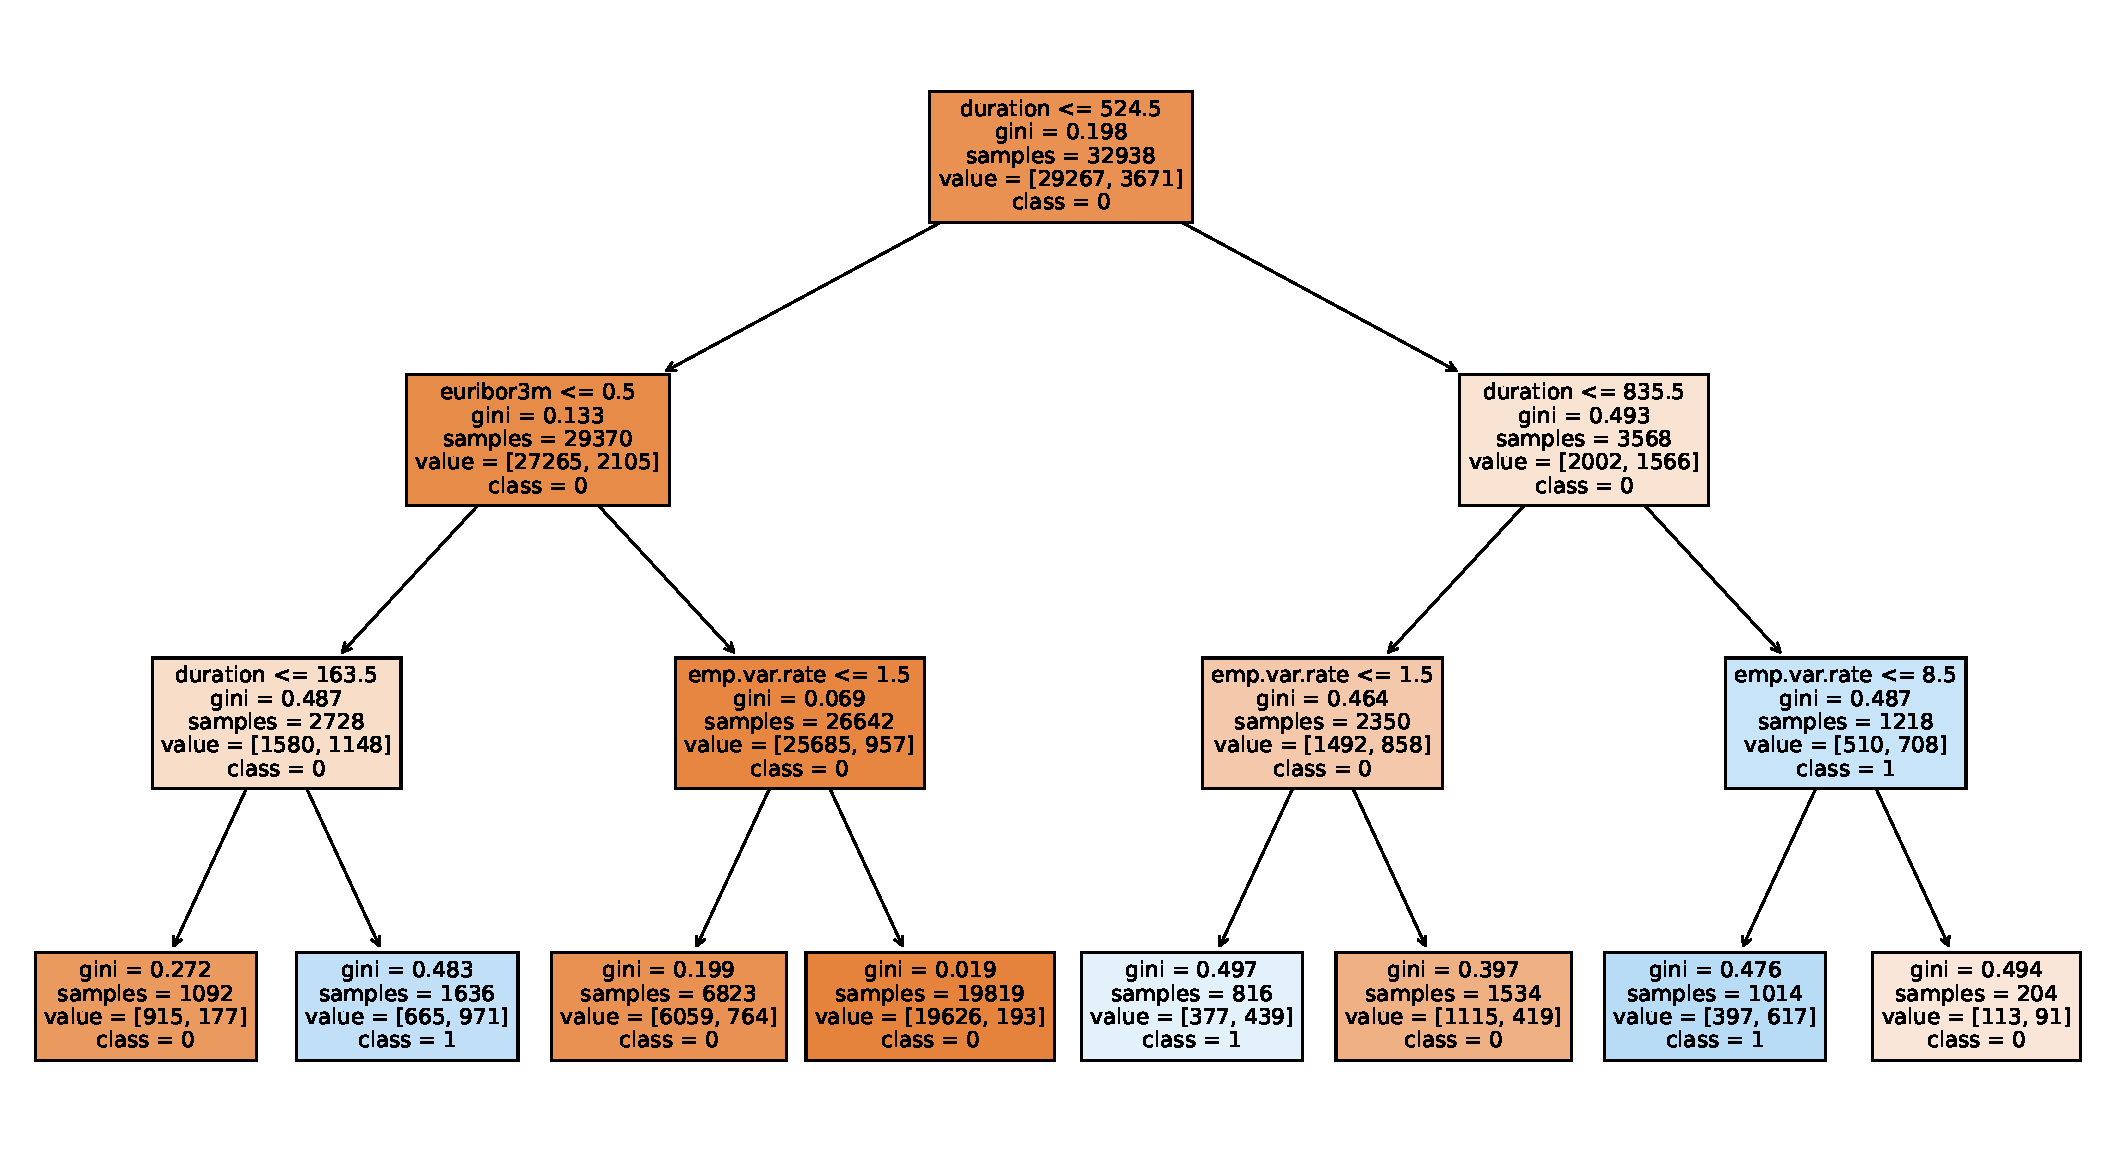
\includegraphics[width=.9\textwidth]{plot/classification/decision_tree.pdf}
    \end{center}
    
    \subsection{Random Forest} \label{random_forest}
    
    
    
    \newpage
    \section{Bibliography}
    \bibliographystyle{plain} % We choose the "plain" reference style
    \bibliography{refs} % Entries are in the refs.bib file

\end{document}